\section{Auswertung}
\label{sec:Auswertung}
Mit der Wheatoneschen Brückenschaltung sollten zwei Unbekannte Widerstände ermittelt werden.
\begin{table}
  \centering
  \caption{Messdaten der Widerstände $R_2$, $R_3$ und $R_4$, für $R_\text{x}$= Wert 10 und $R_\text{x}$= Wert 11}
  \begin{tabular}{s s s s s s}
    \toprule
    &\multicolumn{3}{c}{Wert 10} & \multicolumn{3}{c}{Wert 11}\\
    \cmidrule(lr){1-3}\cmidrule(lr){4-6}
    {}
    
  \end{tabular}
\end{table}
\begin{figure}
  \centering
  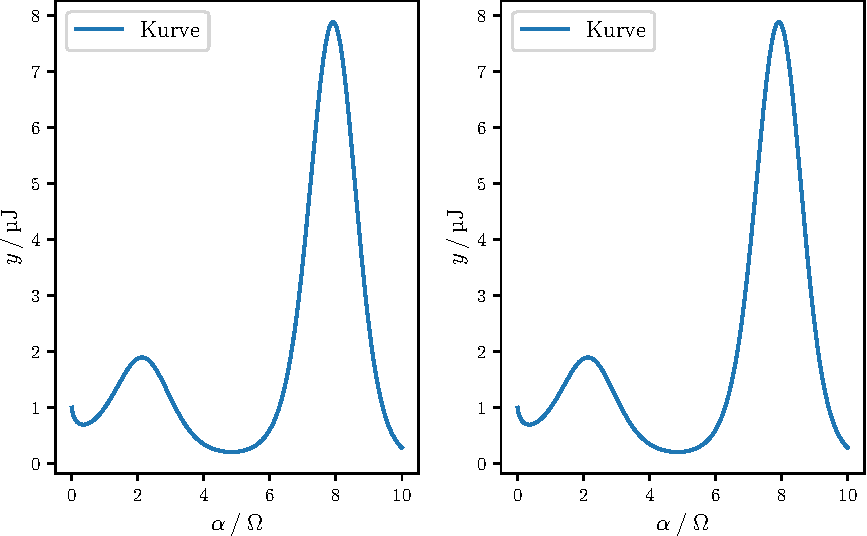
\includegraphics{plot.pdf}
  \caption{Plot.}
  \label{fig:plot}
\end{figure}


Siehe \autoref{fig:plot}!
